% OpenJLS datasheet. Build: tectonic openjls_datasheet.tex
\documentclass[10pt,a4paper]{article}

\usepackage[margin=22mm]{geometry}
\usepackage{amsmath}
\usepackage{graphicx}
\usepackage{booktabs}
\usepackage{array}
\usepackage{tabularx}
\usepackage{xcolor}
\usepackage{enumitem}
\usepackage{fancyhdr}
\usepackage{listings}
\usepackage{tikz}
\usepackage{tikz-timing}
\usepackage[hidelinks]{hyperref}

\graphicspath{{../Images/}}
\setlist{nosep,leftmargin=1.4em}
\newcolumntype{C}{>{\centering\arraybackslash}m{0.10\textwidth}}
\renewcommand{\arraystretch}{1.08}

\definecolor{ojblue}{RGB}{0,80,140}

\lstset{
  basicstyle=\ttfamily\scriptsize,
  keywordstyle=\color{ojblue}\bfseries,
  commentstyle=\color{gray},
  language=VHDL,
  showstringspaces=false,
  frame=single,
  columns=fullflexible,
}

\pagestyle{fancy}
\fancyhf{}
\lhead{\textbf{OpenJLS} — JPEG-LS Encoder IP}
\rhead{Datasheet}
\lfoot{\small v1.0}
\rfoot{\small \thepage}
\renewcommand{\headrulewidth}{0.4pt}

\setcounter{secnumdepth}{1}

\begin{document}

\begin{center}
  {\LARGE\bfseries OpenJLS}\\[2pt]
  {\large JPEG-LS Lossless Encoder IP Core --- Datasheet}\\[2pt]
  {\small Version 1.0 \quad\textbullet\quad Single-component, fully pipelined, vendor-agnostic VHDL}
\end{center}

\vspace{4pt}

%======================================================================
\section{Overview}
OpenJLS is a JPEG-LS (ISO/IEC 14495-1 / ITU-T T.87) lossless encoder for FPGAs.
It encodes single-component (grayscale) images at one pixel per clock with no
external memory, streaming a standards-compliant JPEG-LS bitstream out over
AXI4-Stream. Source, license and the full verification suite are public at
\url{https://github.com/VitorMendesC/OpenJLS}.

\begin{tabularx}{\textwidth}{@{}>{\bfseries}l X@{}}
  \toprule
  Standard      & JPEG-LS lossless (ISO/IEC 14495-1, ITU-T T.87) \\
  Components    & Single (grayscale) \\
  Pixel depth   & 8--16 bits (\texttt{BITNESS}) \\
  Image size    & Up to $65535\times65535$ px, minimum $4\times1$ \\
  Throughput    & 1 pixel / clock \\
  Latency       & 14 clock cycles \\
  $f_{max}$     & $\sim$240\,MHz (Xilinx UltraScale+ \texttt{xczu7eg-1}, RTL-only) \\
  Interface     & AXI4-Stream input (pixels) and output (bitstream) \\
  Memory        & On-chip line buffer, one image row; no external RAM \\
  Resources     & $\sim$8k LUT, $\sim$2.1k FF + BRAM scaling with image width \\
  Portability   & Vendor-agnostic VHDL (open-logic primitives) \\
  \bottomrule
\end{tabularx}

%======================================================================
\section{Functional description}
The core is a fully pipelined encoder with a latency of 14 clock cycles: an
input register, six processing stages (gradient computation, context modeling,
MED prediction with bias correction, Golomb--Rice / run-length coding) and
three internally registered output stages (bit packer, byte stuffer, framer).
End-of-image is derived internally from the configured dimensions; the output
bitstream is self-delimiting.

\begin{center}
  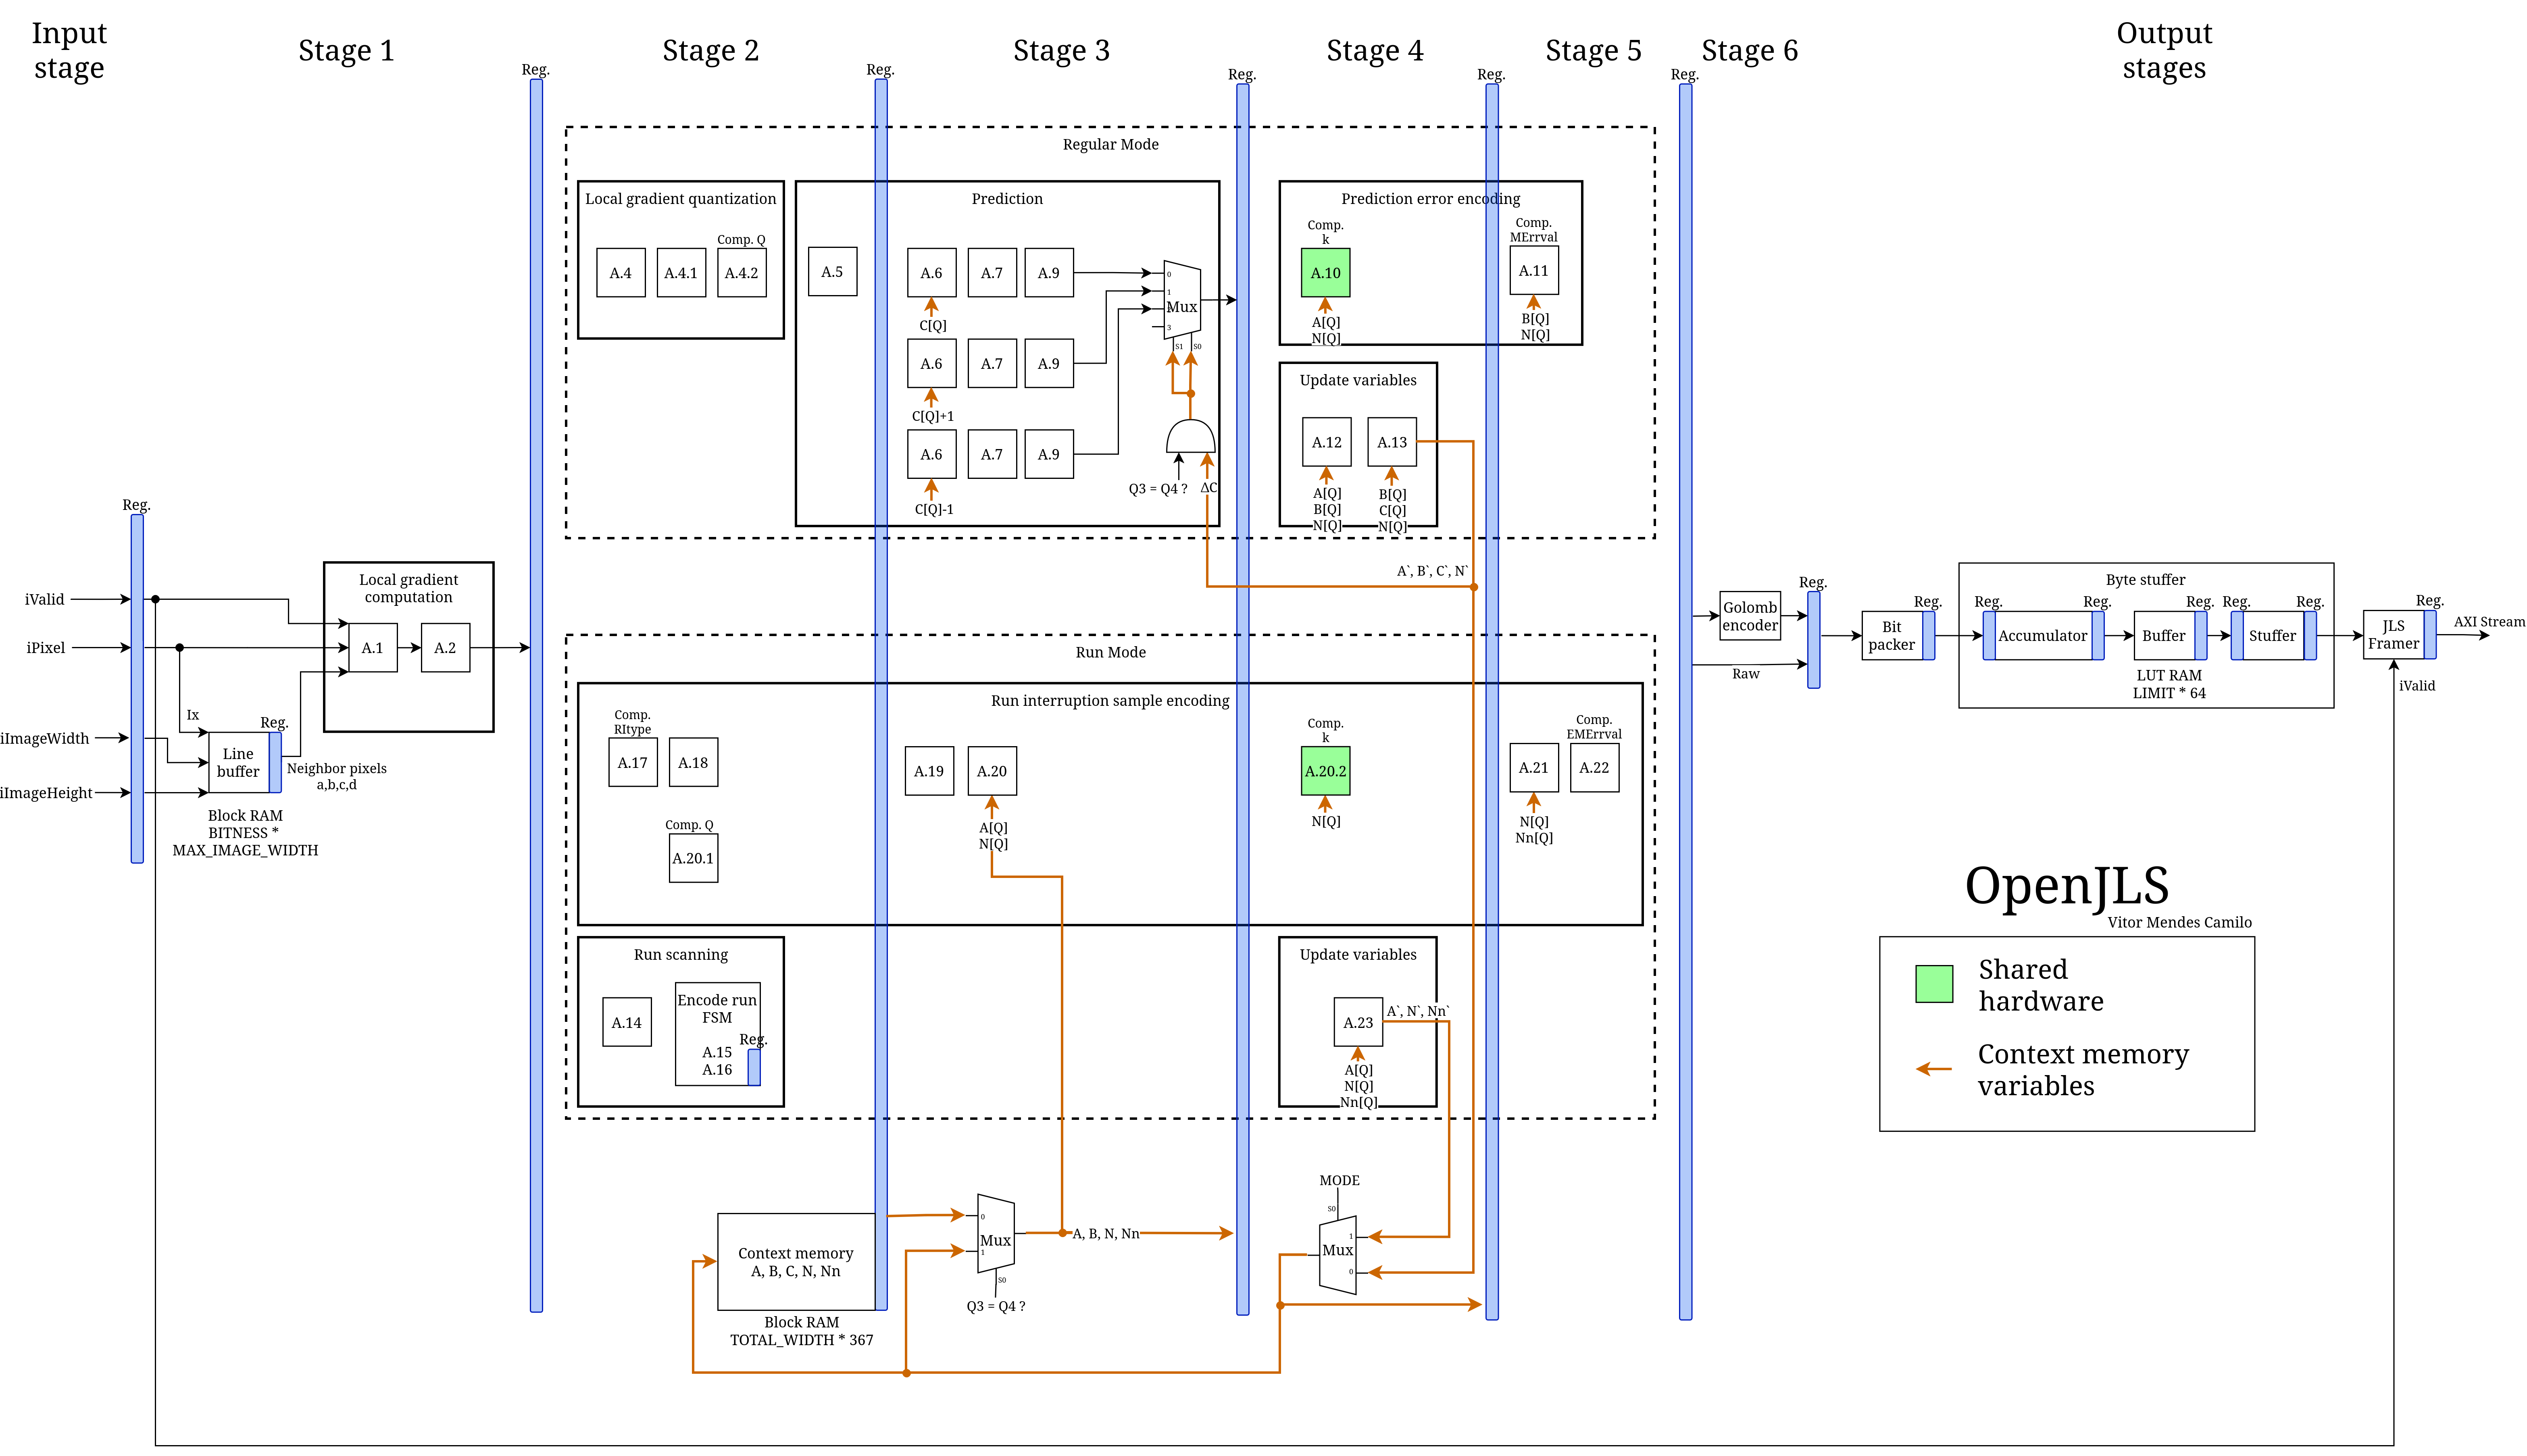
\includegraphics[width=0.80\textwidth]{OpenJLS_arch.png}
\end{center}

%======================================================================
\section{Generics}
\begin{tabularx}{\textwidth}{@{}l C X@{}}
  \toprule
  \textbf{Generic} & \textbf{Range} & \textbf{Description} \\
  \midrule
  \texttt{BITNESS}          & 8--16       & Pixel bit depth. \\
  \texttt{MAX\_IMAGE\_WIDTH}  & 4--65535    & Largest width supported; sets line-buffer depth. \\
  \texttt{MAX\_IMAGE\_HEIGHT} & 1--65535    & Largest height supported. \\
  \texttt{OUT\_WIDTH}        & 48--1024    & Output bus width in bits; multiple of 8. \\
  \bottomrule
\end{tabularx}

%======================================================================
\section{Ports}
All ports are synchronous to the rising edge of \texttt{iClk}. The streaming
ports map one-to-one onto AXI4-Stream as shown.

\begin{tabularx}{\textwidth}{@{}l c l l X@{}}
  \toprule
  \textbf{Port} & \textbf{Dir} & \textbf{Width} & \textbf{AXIS} & \textbf{Role} \\
  \midrule
  \texttt{iClk}        & in  & 1                       & ---             & Clock. \\
  \texttt{iRst}        & in  & 1                       & ---             & Synchronous reset, active high; latches dimensions. \\
  \texttt{iImageWidth} & in  & $\lceil\log_2(\mathrm{MAX\_W}{+}1)\rceil$ & --- & Image width, pixels (configuration). \\
  \texttt{iImageHeight}& in  & $\lceil\log_2(\mathrm{MAX\_H}{+}1)\rceil$ & --- & Image height, pixels (configuration). \\
  \texttt{iValid}      & in  & 1                       & \texttt{TVALID} & Pixel valid. \\
  \texttt{iPixel}      & in  & \texttt{BITNESS}        & \texttt{TDATA}  & Pixel data. \\
  \texttt{oReady}      & out & 1                       & \texttt{TREADY} & Input ready. \\
  \texttt{oData}       & out & \texttt{OUT\_WIDTH}     & \texttt{TDATA}  & Bitstream beat. \\
  \texttt{oValid}      & out & 1                       & \texttt{TVALID} & Output valid. \\
  \texttt{oKeep}       & out & \texttt{OUT\_WIDTH/8}   & \texttt{TKEEP}  & Valid-byte mask on final beat. \\
  \texttt{oLast}       & out & 1                       & \texttt{TLAST}  & End of image. \\
  \texttt{iReady}      & in  & 1                       & \texttt{TREADY} & Downstream ready. \\
  \bottomrule
\end{tabularx}

\noindent The input omits \texttt{TLAST} (optional in AXI4-Stream); house-style
port names map directly onto \texttt{s\_axis}/\texttt{m\_axis} for a thin wrapper.

%======================================================================
\section{Timing and protocol}

\textbf{Pixel input.} A pixel transfers on every cycle where
\texttt{iValid} and \texttt{oReady} are both high. The core asserts
\texttt{oReady} continuously and deasserts it only when the output FIFO fills
under downstream backpressure.

\begin{center}
\begin{tikztimingtable}[timing/slope=0.1,xscale=1.7]
  iClk    & 8{C}        \\
  iPixel  & D{P0} 4D{P1} 2D{P2} D{P3}\\
  iValid  & 8H          \\
  oReady  & HHLLHHHH     \\
\end{tikztimingtable}
\end{center}
\noindent \texttt{P2} is held flat across the stall and accepted when
\texttt{oReady} returns high; no pixel is dropped while \texttt{oReady} is low.

\textbf{Reset and configuration.} The image dimensions are sampled while
\texttt{iRst} is high: present \texttt{iImageWidth} and \texttt{iImageHeight}
and hold them stable across a reset pulse; they latch into the internal
registers on the next clock. Pulse reset again before streaming a new
resolution. Tying the dimension ports to \texttt{0} selects the
\texttt{MAX\_IMAGE\_*} maxima; an out-of-range value falls back to the maximum
with a simulation warning.

\begin{center}
\begin{tikztimingtable}[timing/slope=0.1,xscale=1.45]
  iClk         & 7{C}          \\
  iImageWidth  & D{W0} 6D{W1}  \\
  iImageHeight & D{H0} 6D{H1}  \\
  iRst         & LLLHHLL        \\
  sImageWidth  & 5D{W0} 2D{W1} \\
  sImageHeight & 5D{H0} 2D{H1} \\
\end{tikztimingtable}
\end{center}
\noindent The new size (\texttt{W1}/\texttt{H1}) is driven for several cycles,
then \texttt{iRst} pulses high; the dimensions register one clock after the
reset is sampled.

\textbf{Output.} Beats appear on \texttt{oData}/\texttt{oValid} subject to
\texttt{iReady}; \texttt{oLast} marks the final beat and \texttt{oKeep} flags
its valid bytes. Pipeline latency is 14 clock cycles.

%======================================================================
\section{Resources and performance}
Characterized on Xilinx Zynq UltraScale+ \texttt{xczu7eg-fbvb900-1-e},
Vivado 2025.2, 12-bit, RTL-only (no floorplanning). $f_{max}$ is true fmax
(over-constrained until timing fails); at one pixel/clock $\sim$240\,MHz is
$\sim$240\,Mpixel/s.

\begin{minipage}[t]{0.49\textwidth}
\centering
\textbf{$f_{max}$ (MHz) vs image width}\\[2pt]
\begin{tabular}{@{}r r r@{}}
  \toprule
  Width & Default & Best-of$^\dagger$ \\
  \midrule
  4096  & 226.7 & \textbf{249.2} \\
  8192  & 241.0 & \textbf{248.1} \\
  12288 & 237.8 & \textbf{250.4} \\
  16384 & 201.5 & \textbf{252.0} \\
  32768 & 223.3 & \textbf{242.0} \\
  65535 & 235.0 & \textbf{246.2} \\
  \bottomrule
\end{tabular}
\end{minipage}\hfill
\begin{minipage}[t]{0.49\textwidth}
\centering
\textbf{Resources vs image width}\\[2pt]
\begin{tabular}{@{}r r r r@{}}
  \toprule
  Width & LUT & FF & BRAM \\
  \midrule
  4096  & 7512 & 2055 & 1.5 \\
  8192  & 7545 & 2091 & 3.0 \\
  12288 & 7546 & 2123 & 4.5 \\
  16384 & 7674 & 2137 & 5.5 \\
  32768 & 7636 & 2137 & 11.0 \\
  65535 & 7781 & 2162 & 22.0 \\
  \bottomrule
\end{tabular}
\end{minipage}

\vspace{6pt}
\noindent $^\dagger$Best of three implementation strategies
(\texttt{Congestion\_SpreadLogic\_high}, \texttt{Performance\_NetDelay\_high},
\texttt{Performance\_ExplorePostRoutePhysOpt}); the design is congestion-bound,
so the winning strategy shifts with image size (results are deterministic, so
the per-size winner is a reliable selection). Logic is essentially constant with
image size; only the line-buffer BRAM scales with width and pixel depth.

%======================================================================
\section{Integration example}
\begin{lstlisting}
u_enc : entity work.openjls_top
  generic map (
    BITNESS          => 8,
    MAX_IMAGE_WIDTH  => 4096,
    MAX_IMAGE_HEIGHT => 4096,
    OUT_WIDTH        => 64 )
  port map (
    iClk         => clk,
    iRst         => rst,                  -- hold high while dims are stable
    iImageWidth  => img_w,                -- latched on reset
    iImageHeight => img_h,
    iValid       => px_valid,             -- pixel stream (AXIS slave)
    iPixel       => px_data,
    oReady       => px_ready,
    oData        => m_tdata,              -- bitstream (AXIS master)
    oValid       => m_tvalid,
    oKeep        => m_tkeep,
    oLast        => m_tlast,
    iReady       => m_tready );
\end{lstlisting}

%======================================================================
\section{Conformance and verification}
Verified by simulation with NVC using a layered, self-checking suite run at
both RTL and post-synthesis (gate-level) stages:
\begin{itemize}
  \item \textbf{OSVVM} --- per-module tests against independent T.87-derived
        reference models, plus top-level control-plane stress (reset injection,
        backpressure, randomized sizes) with requirements tracking.
  \item \textbf{Coverage} --- OSVVM functional coverage with NVC structural code coverage (99\%+ statements).
  \item \textbf{Golden model} --- byte-exact vs the independent CharLS C++
        encoder over 287 real and synthetic images, plus ISO/IEC 14495-1 vectors.
  \item \textbf{Design contracts} --- embedded PSL assertions (AXI4-Stream protocol, internal handshakes) on every run.
  \item \textbf{Post-synthesis} --- the stress test and a golden-model subset re-run on the synthesized netlist.
\end{itemize}

\noindent Latest regression snapshot (live, per-test reports at
\url{https://vitormendesc.github.io/OpenJLS/}):

\begin{tabularx}{\textwidth}{@{}l c c X@{}}
  \toprule
  \textbf{Suite} & \textbf{Status} & \textbf{Test/Cov} & \textbf{Summary} \\
  \midrule
  OSVVM suite             & PASS & 100\%  & 36 tests, 129\,810 affirmations (module + top control-plane) \\
  NVC code coverage       & info & 99.2\% & Per-file statement breakdown \\
  Golden model            & PASS & 100\%  & 287/287 images byte-exact vs CharLS \\
  Post-synth OSVVM        & PASS & 100\%  & Control-plane stress on the gate-level netlist \\
  Post-synth golden model & PASS & 100\%  & 156/156 images byte-exact vs CharLS \\
  \bottomrule
\end{tabularx}

%======================================================================
\section*{Revision history}
\begin{tabular}{@{}l l l@{}}
  \toprule
  \textbf{Version} & \textbf{Date} & \textbf{Notes} \\
  \midrule
  1.0 & 2026-06 & Initial release. \\
  \bottomrule
\end{tabular}

\vspace{6pt}
\noindent\textbf{References.}
ITU-T T.87 / ISO/IEC 14495-1;
Y.\,M.\,Mert, \emph{Key Architectural Optimizations for Hardware Efficient
JPEG-LS Encoder}, IEEE 2018;
\href{https://github.com/team-charls/charls}{CharLS};
\href{https://github.com/open-logic/open-logic}{open-logic}.

\end{document}
